\documentclass[a4paper,12pt]{article}
\usepackage[T1,T2A]{fontenc}
\usepackage[utf8]{inputenc}
\usepackage[english,ukrainian]{babel}


\usepackage{ upgreek }
\usepackage{amsmath}

\usepackage{graphicx}
\graphicspath{{./pictures/}}


\usepackage[unicode=true,colorlinks=true,urlcolor=blue,citecolor=green,linkcolor=blue]{hyperref}
\usepackage[ukrainian,nameinlink]{cleveref}
\usepackage{geometry} % Меняем поля страницы
\geometry{left=2cm}% левое поле
\geometry{right=1.5cm}% правое поле
\geometry{top=1cm}% верхнее поле
\geometry{bottom=2cm}% нижнее поле



\begin{document}
	
	\begin{titlepage}
		\vspace*{6cm}
		\begin{center}
			
			\large
			\textbf{Звіт}\\
			\textbf{до лабораторної роботи №2:}\\
			\textbf{<<Чисельне розв'язання рівняння Бюргерса>>}
			
		\end{center}
		
		\vspace{8cm}
		\begin{flushright}
			студента 1-го курсу магістратури\\
			факультету комп'ютерних наук та кібернетики\\
			Кравця Олексія
		\end{flushright}
		
	\end{titlepage}

\newpage
\tableofcontents
\newpage
%document here
\section{Постановка задачі}

Маємо рівняння Бюргерса:
\begin{equation} \label{eq1}
	u_t + \beta u u_x = \gamma u_{xx}
\end{equation}

Де $\gamma u_{xx}$ -- лінійна дифузія, $\gamma >0$ -- коефіцієнт дифузії. Якщо, крім того, відсутня в'язкість, тобто $\gamma \rightarrow 0$, то (\ref{eq1}) є нелінійним хвильовим рівнянням.

Рівняння розглядається у циліндричній області $Q = \left\{ \Omega \times (0 \le t \le T) \right\}$, де $\Omega = \left\{ 0 \le x \le l \right\}$. Маємо наступні початково крайові умови

\begin{equation} \label{eq2}
	\begin{aligned}
		u(x,0) = \phi(x) \\
		u(0,t) = u_1(t) \\
		u(l,t) = u_2 (t)
	\end{aligned}	
\end{equation}

де $\phi(x) \in C^1(R)$та обмежена при $x \rightarrow \infty$.

Для розв'язання використати:
\begin{enumerate}
	\item Неявну різницеву схему
	\item Двокроковий симетризований алгоритм \cite{TwoStep}.
\end{enumerate}

\section{Неявна різницева схема}

Позначимо $u$ -- наближений розв'язок. $h$ -- крок по простору, $\tau$ -- крок по часу.

Позначимо $x_i = ih$, $t_v = v \tau$. Тоді можемо переписати рівняння (\ref{eq1}) у таку різницеву схему

\begin{equation} \label{eq3}
	\frac{u_i^{v+1} - u_i^{v}}{\tau} + \beta u^{v+1}_{i} \frac{u^{v+1}_{i+1} - u^{v+1}_{i-1}}{2h} = \gamma \frac{u^{v+1}_{i+1} - 2 u^{v+1}_{i} + u^{v+1}_{i-1}}{h^2}
\end{equation}

Перепишемо (\ref{eq3}) у більш зручний вигляд

\begin{equation} \label{eq4}
	u^{v+1}_{i} \left(1 + \frac{2 \gamma \tau}{h^2} \right) + \frac{\beta \tau}{2h} u^{v+1}_{i} \left( u^{v+1}_{i+1} - u^{v+1}_{i-1} \right) - \frac{\gamma \tau}{h^2} \left( u^{v+1}_{i+1} + u^{v+1}_{i-1} \right) - u^{v}_{i} =0
\end{equation}

Маємо нелінійне рівняння. Будемо розв'язувати його методом Ньютона:

\subsection{Метод Ньютона}

Нехай маємо деяку вектор-функцію $f(x) = \left(f_1(x), \ldots, f_n(x)\right)$, що двічі неперервно диференційована в деякому околі розв'язку $x^*$ рівняння (системи рівнянь)
\begin{displaymath}
	f(x) = 0
\end{displaymath}

Матриця Якобі $F(x)$:

\begin{displaymath}
	\begin{pmatrix}
	\frac{\partial f_1(x)}{\partial x_1} & \cdots & \frac{\partial f_1(x)}{\partial x_n} \\
	\cdots  & \cdots & \cdots\\
	\frac{\partial f_n(x)}{\partial x_1} & \cdots & \frac{\partial f_n(x)}{\partial x_n} \\
	\end{pmatrix}	
\end{displaymath}

Тоді метод Ньютона має вигляд

\begin{equation} \label{newton_eq}
	x^{k+1} = x^{k} - F^{-1}(x^k) f(x^k), \quad k = 1,2,\ldots
\end{equation}

\subsection{Використання методу Ньютона}

Розглянемо рівняння (\ref{eq4}). Будемо розглядати ліву частину, як функцію для методу Ньютона. Тоді $i$-ий компонент функції має вигляд

\begin{equation} \label{eq5}
	f_i(u^{v+1}) = u_i^{v+1} \left( 1 + \frac{2 \gamma \tau}{h^2} \right) + \frac{\beta \tau}{2h} u^{v+1}_{i} \left( u^{v+1}_{i+1} - u^{v+1}_{i-1} \right) - \frac{\gamma \tau}{h^2} \left( u^{v+1}_{i+1} + u^{v+1}_{i-1} \right) - u^{v}_{i} =0
\end{equation}

Можемо записати матрицю Якобі, вона тридіагональна.

Перший рядок має вигляд
\begin{displaymath}
	\begin{bmatrix}
		\left(1 + \frac{2 \gamma \tau}{h^2} \right)+  \frac{\beta \tau}{2h} \left( u^{v+1}_{2} - u_{1}(t_v+\tau)\right), & \frac{\beta \tau}{2h} u_1^{v+1} - \frac{\gamma \tau}{h^2}, & \cdots
	\end{bmatrix}
\end{displaymath}

$i$-ий рядок має вигляд
\begin{displaymath}
	\begin{bmatrix}
 	 \cdots & -\frac{\beta \gamma}{2h} u^{v+1}_{i} - \frac{\gamma \tau}{h^2}, & \left( 1 + \frac{2 \gamma \tau}{h^2} \right) +  \frac{\beta \tau}{2h} \left( u^{v+1}_{i+1} - u_{i-1}^{v+1}\right), & \frac{\beta \gamma}{2h} u_{i}^{v+1} - \frac{\gamma \tau}{h^2}, & \cdots	
	\end{bmatrix}	
\end{displaymath}

Останній рядок
\begin{displaymath}
\begin{bmatrix}
\cdots & - \frac{\beta \gamma}{2h} u_{n}^{v+1} - \frac{\gamma \tau}{h^2}, & \left( 1 + \frac{2\gamma \tau}{h^2} \right) + \frac{\beta \tau}{2h} \left( u_2(t_v+\tau) - u_{n-1}^{v+1} \right)
\end{bmatrix}	
\end{displaymath}

\section{Двокроковий симетризований алгоритм}

Позначення не змінилися. Додамо позначення $c$ - кількість пройдених алгоритмом кроків. Також додамо таке позначення
\begin{equation} \label{eq6}
		L u_{i}^{v} \equiv - \beta u_{i}^{v} \frac{u_{i+1}^{v} - u_{i-1}^{v}}{2h} + \gamma \frac{u_{i+1}^{v} - 2u_{i}^{v} +u_{i-1}^{v}}{h^2}
\end{equation}

Візьмемо точки $u_{i}$, що задовольняють умові: $(i+c)$ ділиться на 2. Будемо оновлювати їх за явної різницевою схемою.

\begin{equation} \label{eq7}
	u_i^{v+1}= u_i^{v} + \tau Lu_{i}^{v}
\end{equation}

Після цього розглянемо точки, що залишилися, вони задовольняють умові: $(i+c)$ не ділиться на 2. Будемо оновлювати їх за неявно різницевою схемою, завдяки рівнянню (\ref{eq7}) можна буде явним чином отримати $u_{i}^{v+1}$.

\begin{equation} \label{eq8}
u_i^{v+1}= u_i^{v} + \tau Lu_{i}^{v+1}
\end{equation}

Розпишемо рівняння (\ref{eq8}), підставляючи в нього (\ref{eq6}), для того, щоб явно вивести $u_i^{v+1}$

\begin{equation} \label{eq9}
	u^{v+1}_{i} = \frac{u_i^v + \frac{\gamma \tau}{h^2} \left( u^{v+1}_{i+1} + u^{v+1}_{i-1} \right) }{1 + \frac{\beta \tau}{2h} \left( u^{v+1}_{i+1} - u^{v+1}_{i-1} \right) + \frac{2 \gamma \tau}{h^2} }
\end{equation}

Ця схема абсолютна стійка, та більш точна на парних часових кроках.

\section{Обчислювальний експеримент}

Проведемо обчислювальний експеримент з параметрами: $\beta = 1$,$\gamma=1$, $T = 50$. Функції $\phi(x), u_1(x), u_2(x)$ обрати у відповідності до точного розв'язку $u^*(x,t) = f(x - ct)$, де 

\begin{equation} \label{eq10}
	f(x) = u_{02} + \frac{u_{01} - u_{02}}{1 + \exp\left(\frac{(u_{01}-u_{02})\cdot x }{2\gamma} \right)}
\end{equation}

Де $c = (u_{01} + u_{02})/2$, де $u_{01} = 3, u_{02} = 1$.

\begin{figure}[ht]
	\center{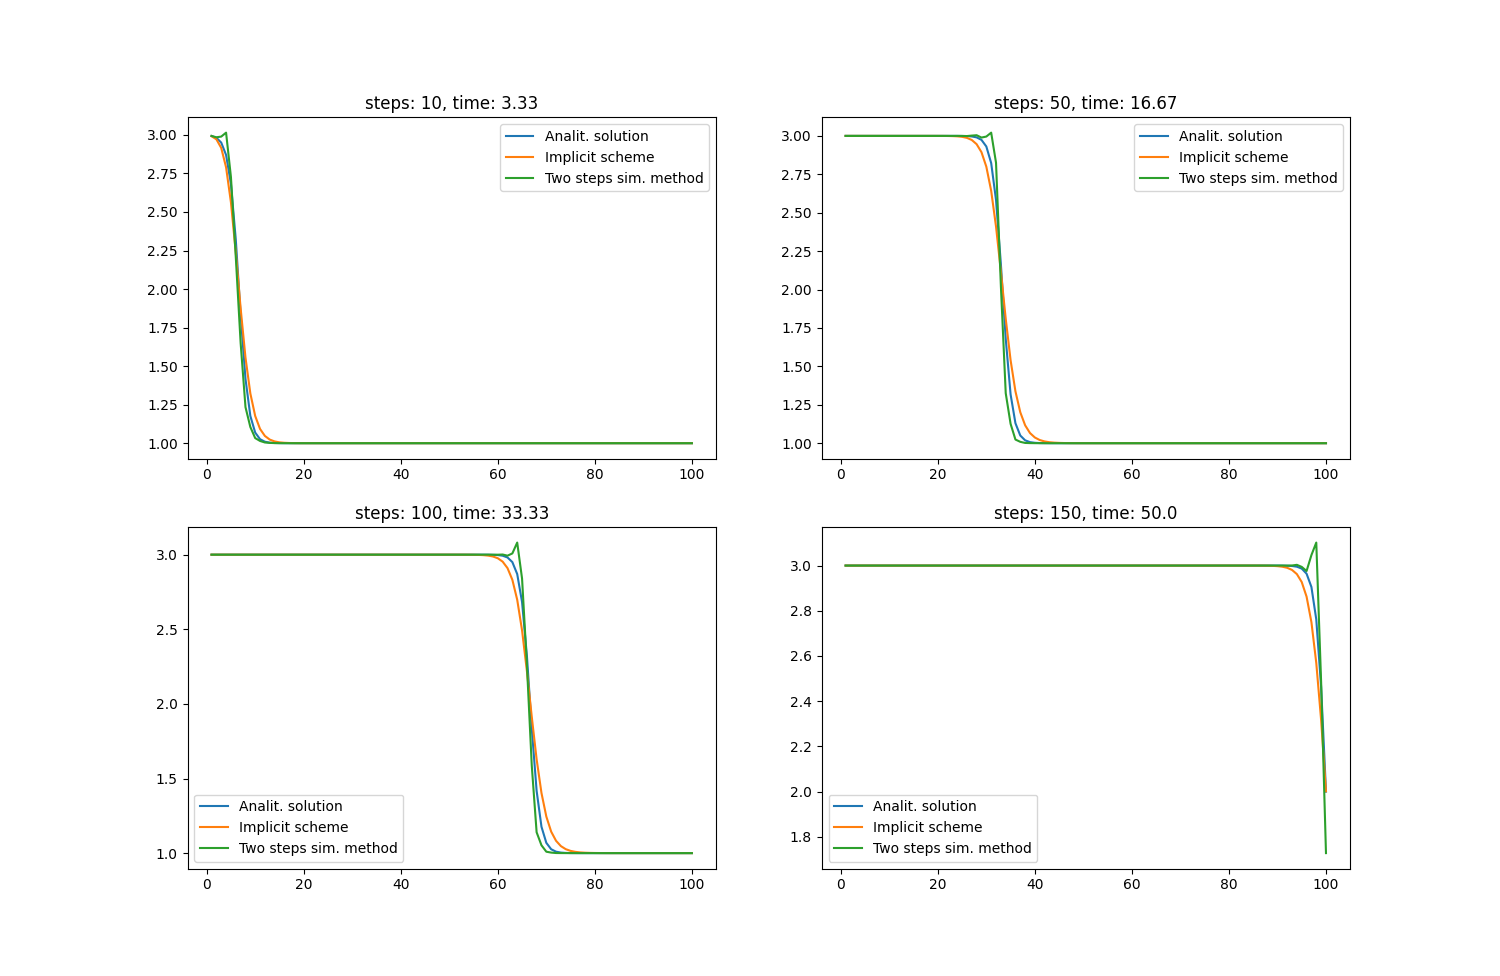
\includegraphics[width=1\linewidth]{Figure_1.png}}
	\caption{Графіки розв'язку}
	\label{fig:sss1}
\end{figure}

Анімацію розв'язку можна переглянути за  \href{https://github.com/AlKravets/Numerical-model-of-dynamics-of-systems/blob/master/lab2/gif/res_animation.gif}{посиланням}.

Таблиця помилок на кроках, що зображені на графіках. $N$ -- кількість кроків. Значення в таблиці -- абсолютна помилка.

\begin{tabular}{| c | c | c | c | c |}
	\hline
	$N$  &  10 & 50 & 100 & 150 \\
	\hline
	Неявна різницева схема & 0.1462 & 0.2226 & 0.2262 & 0.1924 \\
	Двокроковий симетризований алгоритм & 0.1846 & 0.3533 & 0.2775 & 0.3402 \\
	\hline
\end{tabular}


\section{Висновки}
В роботі були реалізовані методи чисельного розв'язання рівняння Бюргерса, був проведений чисельний експеримент. Одержані результати показують, що двокроковий симетризований алгоритм має апроксимаційні властивості подібні до неявної різницевої схеми, проте він не потребує розв'язання нелінійного рівняння на кожному кроці.


\addcontentsline{toc}{section}{Література}
\begin{thebibliography}{}
	\bibitem{TwoStep} Олександр Ю. Грищенко, В’ячеслав В. Оноцький. Двокроковий різницевий алгоритм для рівняння Бюргерса. 2007, <<Вісник Київського університету>>
	\bibitem{Volkov}  Е.А.Волков Численные методы, 1987, Москва <<Наука>>
\end{thebibliography}

\end{document}
